\tinysidebar{\debug{exercises/{tiling0/answer.tex}}}
The following
{\small \begin{console}[frame=single,fontsize=\small]
[student@localhost 350-hashtable] g++ main.cpp; ./a.out
hash of
42: 42
42: 42
-1: 18446744073709551615
3.14: 5464867211497793177
0.0: 6369015886390043782
'a': 97
true: 1
"hello world": 5577293430985752569
\end{console}
}

\begin{center}
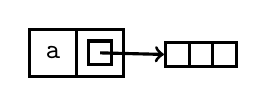
\begin{tikzpicture}

\draw (0.3, 0.3)
  node[draw, line width=0.04cm, , color=black,
       rounded corners=0cm, inner sep=0cm] {

\begin{minipage}[t][0.6cm]{0.6cm}
\mbox{}

\end{minipage}

};\draw (0.3, 0.3) node[color=black] {{\texttt{a}}};
\draw (0.8999999999999999, 0.3)
  node[draw, line width=0.04cm, , color=black,
       rounded corners=0cm, inner sep=0cm] {

\begin{minipage}[t][0.6cm]{0.6cm}
\mbox{}

\end{minipage}

};
\draw (0.9, 0.3)
  node[draw, line width=0.04cm, , color=black,
       rounded corners=0cm, inner sep=0cm] {

\begin{minipage}[t][0.3cm]{0.3cm}
\mbox{}

\end{minipage}

};
\draw (1.88, 0.28)
  node[draw, line width=0.04cm, , color=black,
       rounded corners=0cm, inner sep=0cm] {

\begin{minipage}[t][0.3cm]{0.3cm}
\mbox{}

\end{minipage}

};
\draw (2.1799999999999997, 0.28)
  node[draw, line width=0.04cm, , color=black,
       rounded corners=0cm, inner sep=0cm] {

\begin{minipage}[t][0.3cm]{0.3cm}
\mbox{}

\end{minipage}

};
\draw (2.48, 0.28)
  node[draw, line width=0.04cm, , color=black,
       rounded corners=0cm, inner sep=0cm] {

\begin{minipage}[t][0.3cm]{0.3cm}
\mbox{}

\end{minipage}

};\draw[line width=0.04cm,black,->] (0.9,0.3) to  (1.71,0.28);
\end{tikzpicture}

\end{center}


can be completed with tilings of 2-by-$(n-1)$ tilings.
All these complete tilings are distinct.
The number of such tilings is $2 a_{n-1}$.

The following
\begin{center}
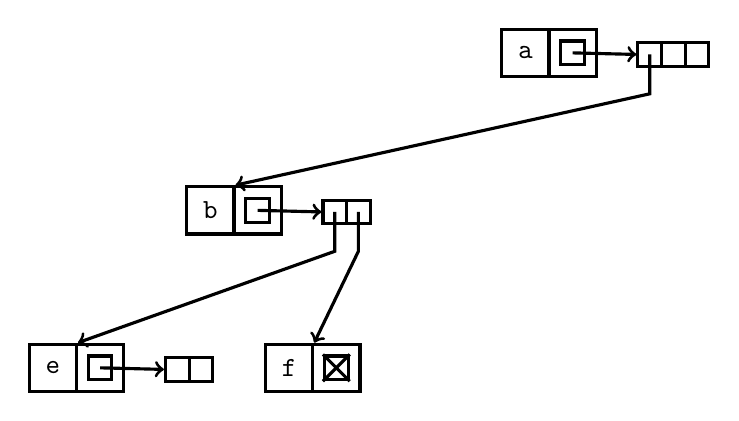
\begin{tikzpicture}

\draw (0.3, 0.3)
  node[draw, line width=0.04cm, , color=black,
       rounded corners=0cm, inner sep=0cm] {

\begin{minipage}[t][0.6cm]{0.6cm}
\mbox{}

\end{minipage}

};\draw (0.3, 0.3) node[color=black] {{\texttt{a}}};
\draw (0.8999999999999999, 0.3)
  node[draw, line width=0.04cm, , color=black,
       rounded corners=0cm, inner sep=0cm] {

\begin{minipage}[t][0.6cm]{0.6cm}
\mbox{}

\end{minipage}

};
\draw (0.9, 0.3)
  node[draw, line width=0.04cm, , color=black,
       rounded corners=0cm, inner sep=0cm] {

\begin{minipage}[t][0.3cm]{0.3cm}
\mbox{}

\end{minipage}

};
\draw (1.88, 0.28)
  node[draw, line width=0.04cm, , color=black,
       rounded corners=0cm, inner sep=0cm] {

\begin{minipage}[t][0.3cm]{0.3cm}
\mbox{}

\end{minipage}

};
\draw (2.1799999999999997, 0.28)
  node[draw, line width=0.04cm, , color=black,
       rounded corners=0cm, inner sep=0cm] {

\begin{minipage}[t][0.3cm]{0.3cm}
\mbox{}

\end{minipage}

};
\draw (2.48, 0.28)
  node[draw, line width=0.04cm, , color=black,
       rounded corners=0cm, inner sep=0cm] {

\begin{minipage}[t][0.3cm]{0.3cm}
\mbox{}

\end{minipage}

};\draw[line width=0.04cm,black,->] (0.9,0.3) to  (1.71,0.28);

\draw (-3.6999999999999997, -1.7)
  node[draw, line width=0.04cm, , color=black,
       rounded corners=0cm, inner sep=0cm] {

\begin{minipage}[t][0.6cm]{0.6cm}
\mbox{}

\end{minipage}

};\draw (-3.6999999999999997, -1.7) node[color=black] {{\texttt{b}}};
\draw (-3.0999999999999996, -1.7)
  node[draw, line width=0.04cm, , color=black,
       rounded corners=0cm, inner sep=0cm] {

\begin{minipage}[t][0.6cm]{0.6cm}
\mbox{}

\end{minipage}

};
\draw (-3.0999999999999996, -1.7)
  node[draw, line width=0.04cm, , color=black,
       rounded corners=0cm, inner sep=0cm] {

\begin{minipage}[t][0.3cm]{0.3cm}
\mbox{}

\end{minipage}

};
\draw (-2.12, -1.7200000000000002)
  node[draw, line width=0.04cm, , color=black,
       rounded corners=0cm, inner sep=0cm] {

\begin{minipage}[t][0.3cm]{0.3cm}
\mbox{}

\end{minipage}

};
\draw (-1.8199999999999998, -1.7200000000000002)
  node[draw, line width=0.04cm, , color=black,
       rounded corners=0cm, inner sep=0cm] {

\begin{minipage}[t][0.3cm]{0.3cm}
\mbox{}

\end{minipage}

};\draw[line width=0.04cm,black,->] (-3.1,-1.7) to  (-2.29,-1.72);

\draw (-5.7, -3.6999999999999997)
  node[draw, line width=0.04cm, , color=black,
       rounded corners=0cm, inner sep=0cm] {

\begin{minipage}[t][0.6cm]{0.6cm}
\mbox{}

\end{minipage}

};\draw (-5.7, -3.6999999999999997) node[color=black] {{\texttt{e}}};
\draw (-5.1, -3.6999999999999997)
  node[draw, line width=0.04cm, , color=black,
       rounded corners=0cm, inner sep=0cm] {

\begin{minipage}[t][0.6cm]{0.6cm}
\mbox{}

\end{minipage}

};
\draw (-5.1, -3.7)
  node[draw, line width=0.04cm, , color=black,
       rounded corners=0cm, inner sep=0cm] {

\begin{minipage}[t][0.3cm]{0.3cm}
\mbox{}

\end{minipage}

};
\draw (-4.119999999999999, -3.72)
  node[draw, line width=0.04cm, , color=black,
       rounded corners=0cm, inner sep=0cm] {

\begin{minipage}[t][0.3cm]{0.3cm}
\mbox{}

\end{minipage}

};
\draw (-3.8199999999999994, -3.72)
  node[draw, line width=0.04cm, , color=black,
       rounded corners=0cm, inner sep=0cm] {

\begin{minipage}[t][0.3cm]{0.3cm}
\mbox{}

\end{minipage}

};\draw[line width=0.04cm,black,->] (-5.1,-3.7) to  (-4.29,-3.72);

\draw (-2.7, -3.6999999999999997)
  node[draw, line width=0.04cm, , color=black,
       rounded corners=0cm, inner sep=0cm] {

\begin{minipage}[t][0.6cm]{0.6cm}
\mbox{}

\end{minipage}

};\draw (-2.7, -3.6999999999999997) node[color=black] {{\texttt{f}}};
\draw (-2.1, -3.6999999999999997)
  node[draw, line width=0.04cm, , color=black,
       rounded corners=0cm, inner sep=0cm] {

\begin{minipage}[t][0.6cm]{0.6cm}
\mbox{}

\end{minipage}

};
\draw (-2.1, -3.7)
  node[draw, line width=0.04cm, , color=black,
       rounded corners=0cm, inner sep=0cm] {

\begin{minipage}[t][0.3cm]{0.3cm}
\mbox{}

\end{minipage}

};\draw[line width=0.04cm,black] (-2.27,-3.53) to  (-1.93,-3.87);
\draw[line width=0.04cm,black] (-1.93,-3.53) to  (-2.27,-3.87);
\draw[line width=0.04cm,black,->] (1.88,0.28) to  (1.88,-0.22) to  (-3.38,-1.38);
\draw[line width=0.04cm,black,->] (-2.12,-1.72) to  (-2.12,-2.22) to  (-5.38,-3.38);
\draw[line width=0.04cm,black,->] (-1.82,-1.72) to  (-1.82,-2.22) to  (-2.38,-3.38);
\end{tikzpicture}

\end{center}



\begin{center}
\begin{tikzpicture}[>=triangle 60,shorten >=0.5pt,node distance=2cm,auto,initial text=, double distance=2pt]
\node[state] (A) at (  0,  0) {$\{q_0\}$};
\node[state] (B) at (  3,  0) {$\{\}$};

\path[->]

;
\end{tikzpicture}
\end{center}
    


\begin{longtable}{|r||r|r|r|r|r|}
\hline 
         & $w_1$ & $w_2$ & $w_3$ & $w_4$ & $\ldots$ \\ \hline \hline 
$M_1$    &       &       &       &       &          \\ \hline 
$M_2$    &       &       &       &       &          \\ \hline 
$M_3$    &       &       &       &       &          \\ \hline 
$M_4$    &       &       &       &       &          \\ \hline 
$\ldots$ &       &       &       &       &          \\ \hline 
\end{longtable}
        


\begin{longtable}{|r||r|r|r|r|r|}
\hline 
         & $w_1$ & $w_2$ & $w_3$ & $w_4$ & $\ldots$ \\ \hline \hline 
$M_1$    & 0     & 0     & 1     & 0     & ...      \\ \hline 
$M_2$    & 1     & 0     & 1     & 1     & ...      \\ \hline 
$M_3$    & 0     & 1     & 1     & 1     & ...      \\ \hline 
$M_4$    & 1     & 0     & 1     & 1     & ...      \\ \hline 
$\ldots$ &       &       &       &       &          \\ \hline 
\end{longtable}
        

can be completed with tilings of 2-by-$(n-2)$ tilings.
All these complete tilings are distinct.
The number of such tilings is $4 a_{n-2}$.

Hence
\[
a_n = 2 a_{n-1} + 4 a_{n-2} \,\,\,\,\, \text{ if } n \geq 2
\]
Furthermore, from the above, we see that $a_1 = 2$ and $a_2 = 4$.
We can compute $a_0$ from the recurrence relation:
\[
a_2 = 2 a_{1} + 4 a_{0}
\]
Therefore
$a_0 = 0$.
Hence we have
\begin{align*}
  a_n =
  \begin{cases}
    0                   & \text{ if } n = 0 \\
    2                   & \text{ if } n = 1 \\
    2 a_{n-1} + 4 a_{n-2} & \text{ if } n \geq 2
  \end{cases}
\end{align*}
